\documentclass[a4paper,11pt]{article}

\usepackage{graphicx}
\usepackage{amsmath}
\usepackage{blindtext}
\usepackage{apacite}
\usepackage{tabularx}
\usepackage{multirow}
\usepackage{geometry}
	\geometry{
	margin = 1in
}
\usepackage{pdflscape}
\usepackage{fancyhdr}
	\pagestyle{fancy}
	\lhead{}
	\chead{}
	\rhead{}
	\lfoot{}
	\cfoot{}
	\rfoot{\thepage}
	\renewcommand{\headrulewidth}{0pt}
\usepackage[T1]{fontenc}
\usepackage[math]{iwona}
\usepackage{mathptmx}
\usepackage{longtable}
\usepackage{caption}
	\setlength{\abovecaptionskip}{0.5em}

\title{\Huge{ENG2016: Bike Project}}
\author{\begin{tabular}{l c}
		Ivan Mihajlovic&2239242 \\
		William Ely&2292204 \\
		Qiyu Zhang&2295435 \\
		Ewan Walker&2235937 \\
		Eduard Fiedler&2248902 \\
\end{tabular}
}
\date{2018}

\linespread{1.25}

\renewcommand{\contentsname}{Table of Contents}

\begin{document}

\pagenumbering{roman}

\begin{titlepage}

	\vspace*{\fill}
    	\begin{center}
		\LARGE{\textsc{University of Glasgow}}\vspace{2em} \\

		\hrulefill\\
		\vspace{0.8em} 
		\Huge{ENG2016: Bike Project}\\\hrulefill
		\vspace{2em}\\
		\LARGE{
			\textsc{Group 23}\vspace{2em}\\
			\begin{tabular}{l c}
				Ivan Mihajlovic\phantom{W}&2239242 \\
				William Ely&2292204 \\
				Qiyu Zhang&2295435 \\
				Ewan Walker&2235937 \\
				Eduard Fiedler&2248902 \\
			\end{tabular}}\\
    	\end{center}
    	\vspace*{\fill}
	\vspace{10em} 

\end{titlepage}

\setcounter{page}{2}

\section*{Abstract}
\addcontentsline{toc}{section}{Abstract}

The purpose of this project is to design an electric bicycle for 55+-year-old men. The goal is to provide insight on the thought process and decision making behind the final design, and how it will be implemented into the current market. This has been done by examining the growing market of electric bikes, and applying sufficient research, in order to construct a realistic bicycle. After analysing multiple different concepts, it was concluded that a men�s Dutch style bike was the ideal design as it allowed a stylish, and comfortable means of commute, in comparison to alternatives.

\pagebreak

\tableofcontents

\pagebreak

\listoftables
\addcontentsline{toc}{section}{List of Tables}

\pagebreak

\listoffigures
\addcontentsline{toc}{section}{List of Figures}

\pagebreak

\pagenumbering{arabic}

\section{Introduction}

With a growing interest in battery powered transportation devices, the electric bicycle has experienced a worldwide, rapid growth in popularity since 1998 \cite{wein07}. However, many companies try to sell their product as an athletic alternative, this caters towards young to middle-aged adults (20-40 years old), and neglects the older population. 

The aim is to design an e-bike that accommodates an older audience by reducing effort, emphasising ergonomics, and improving the quality of their commute. The final product is targeted towards a male market, above the age of 55, and will provide these characteristics in an exceptional manner.

This report will convey the emulation of a typical design process, the means used to conduct decisions for the final design, and its implementation into the current market.

\section{Project Planning}

In order to remain organised, a Gantt chart was formulated. The Gantt chart allowed a visualisation of work allocations for the various topics that were required to complete the project. 

\subsection{Initial Work Allocations}

\begin{table}[!ht]
	\centering
	\caption{Initial Gantt chart}
	\begin{tabular}{l || c  c  c  c  c  c  c  c  c  c  c }
		\multicolumn{1}{l||}{Task}&W1&W2&W3&W4&W5&W6&W7&W8&W9&W10&W11\\\hline\hline
		Research&&&\multicolumn{1}{|c|}{\footnotesize{ALL}}&&&&&&&&\\ \hline
		PDS&&&\multicolumn{2}{|c|}{\footnotesize{ALL}}&&&&&&&\\\hline
		Concept Generation&&&&\multicolumn{2}{|c|}{\footnotesize{ALL}}&&&&&&\\\hline
		CAD&&&&&\multicolumn{3}{|c}{\footnotesize{EW-ED-IV}}&\multicolumn{1}{|c}{\phantom{.}}&&&\\\hline
		Market Analysis&&&&&\multicolumn{2}{|c|}{\footnotesize{QIYU}}&&&&&\\\hline
		House of Quality&&&&&&\multicolumn{2}{|c}{\footnotesize{WILLIAM}}&\multicolumn{1}{|c}{\phantom{.}}&&&\\\hline
		Report&&&&&&&&\multicolumn{4}{|c}{\footnotesize{ALL}}\\\hline
		Presentation&&&&&&&&\multicolumn{4}{|c}{\footnotesize{ALL}}\\\hline
		Group Meetings&&\multicolumn{10}{|c}{\footnotesize{ALL}}
	\end{tabular}
\end{table}

In terms of initial work distribution, the complexity of each topic was allocated between the group members based on: background, and abilities. This required the distribution of the CAD work amongst 3 people, as it was speculated to take longer. Furthermore, in the initial stages group work was emphasised to integrate individual concepts, and weekly meetings were scheduled in order to remain on the same page.

\subsection{Final Work Allocations}

As progress was made with the project, initial roles couldn't be maintained due to different individual schedules. Additionally, by further expanding on the generalised topics in the previous chart, the work had to be allocated differently. This resulted in the following work distribution in order to complete the project on time.

\begin{table}[!ht]
	\centering
	\caption{Final Gantt chart}
	\begin{tabular}{ l || c  c  c  c  c  c  c  c  c  c  c }
		\multicolumn{1}{l||}{Task}&W1&W2&W3&W4&W5&W6&W7&W8&W9&W10&W11\\\hline\hline
		PDS&&&\multicolumn{3}{|c|}{\footnotesize{ALL}}&&&&&&\\\hline
		Concept Designs&&&\multicolumn{2}{|c}{\footnotesize{ALL}}&\multicolumn{1}{|c}{\phantom{.}}&&&&&\\\hline
		Biomechanics&&&&&\multicolumn{5}{|c|}{\footnotesize{QI}}&\\\hline
		Market Analysis&&&&&\multicolumn{5}{|c|}{\footnotesize{WILLIAM}}&\\\hline
		House of Quality&&&&&\multicolumn{5}{|c|}{\footnotesize{EDUARD}}&\\\hline
		Detailed Sketches&&&&&\multicolumn{3}{|c|}{\footnotesize{ALL}}&&&\\\hline
		Components&&&&&\multicolumn{1}{|c}{\footnotesize{ALL}}&\multicolumn{4}{|c|}{\footnotesize{IVAN}}&\\\hline
		Materials&&&&&&\multicolumn{4}{|c|}{\footnotesize{IVAN}}&\\\hline
		Design Analysis&&&&&&&\multicolumn{2}{|c|}{\footnotesize{ALL}}&&&\\\hline
		CAD&&&&&\multicolumn{5}{|c|}{\footnotesize{EWAN}}&\\\hline
		Costing&&&&&&&\multicolumn{3}{|c|}{\footnotesize{IVAN}}&&\\\hline
		Group Meetings&&\multicolumn{10}{|c}{\footnotesize{ALL}}\\\hline
		Presentation&&&&&&&&\multicolumn{4}{|c}{\footnotesize{ALL}}\\\hline
		Report&&&&&&&&\multicolumn{4}{|c}{\footnotesize{ALL}}\\\hline
		Evaluation&&&&&&&&&&&\multicolumn{1}{|c}{\footnotesize{ALL}}
	\end{tabular}
\end{table}

\section{Product Design Specification (User Requirements)}

\section{Biomechanics}

\section{Current Market Analysis}

\section{Conceptual Design}

\subsection{Initial Sketches}

\subsection{Morphological Analysis}

\section{Quality Function Deployment}

In order to meet customer demands, research and initial product specifications are combined to form the House of Quality. The aim is to produce a customer driven product which will fulfil key demands, by translating user requirements into engineering requirements. Then, by comparing the individual aspects, the importance can be visualised and securely compromised if they are deemed unimportant to the design.

\subsection{Engineering Specifications}

\begin{table}[!ht]
	\centering
	\caption{Translation of user requirements}
	\begin{tabular}{l l l r}
		\hline
		Category&User Requirements&Engineering Specifications&Ref\\\hline
	Performance&Bike parts will last for a long time&Fatigue Limit Cycles&1\\
		&Adequate gearing for a city environment&Number of Gears&2\\
		&Mobility at moderate speeds&Turning radius at 20km/h&3\\
		&Temperature resistant&Melting point of Material&4\\
		&Corrosion resistant&Based on material selection&5\\
		&Luggage space&Amount of suitcases supported&6\\
		&High acceleration from rest&Effort required for acceleration&7\\
		&Low-effort for commute&Effort required for distance&8\\
		&Supports the weight of the rider&Material yield strength&9\\
		&Good braking&Braking distance from max speed&10\\
		&Low centre of gravity&Height of C.o.G. above ground&11\\\hline
	Battery&High battery capacity/battery lifespan&Battery capacity&12\\
		&Battery assists up to specified speed&Input choked at certain speed&13\\
		&Battery recharges quickly&Recharge cycle time (full)&14\\
		&Battery supports significant power&Work input&15\\\hline
	Suspension&No deformations due to vibrations&Material yield strength&16\\
		&Remains steady at high speeds&Structural vibrations&17\\
		&Smooth ride&Spring stiffness&18\\\hline
	Ergonomics&Comfortable riding position&Amount of satisfied people&19\\
		&Height adjustable seat and handlebars&Range of adjustment&20\\
		&Easy to assemble&Assembly time&21\\
		&Easy to maintain&Amount of tools required&22\\
		&Easy to carry&Overall weight of bicycle&23\\
	\end{tabular}
\end{table}

When translating user requirements to engineering specifications, various methods of testing and measuring are used to describe them. In terms of performance, properties of the general structure of the bike, and its functionality are considered. Furthermore for the battery and the suspension, these characteristics were considered outside of the performance, as they are aspects that must be well defined for the end design of the bike. Lastly, requirements categorised as ergonomics, are quantified in terms of ease of use and comfort.

\subsection{Analysis}

To form the House of Quality, the following investigations were made to find relationships between the requirements:
\begin{itemize}
	\setlength{\itemsep}{0pt}
	\item What vs. How? (User requirements vs. Engineering specifications)
	\item How vs. How? (Engineering specifications vs. Engineering specifications)
	\item Who vs. What? (Potential buyers vs. User requirements)
	\item Now vs. What? (Similar products on the market vs. User requirements)
	\item How much? (What are the feasible targets in terms of engineering specifications)
\end{itemize}

In the first phase of analysis, User requirements and Engineering specifications are inspected for relationships.

\newpage

\newgeometry{margin=1cm}
\thispagestyle{empty}
\begin{landscape}

\begin{table}[ht]
	\centering
	\caption{House of Quality}
	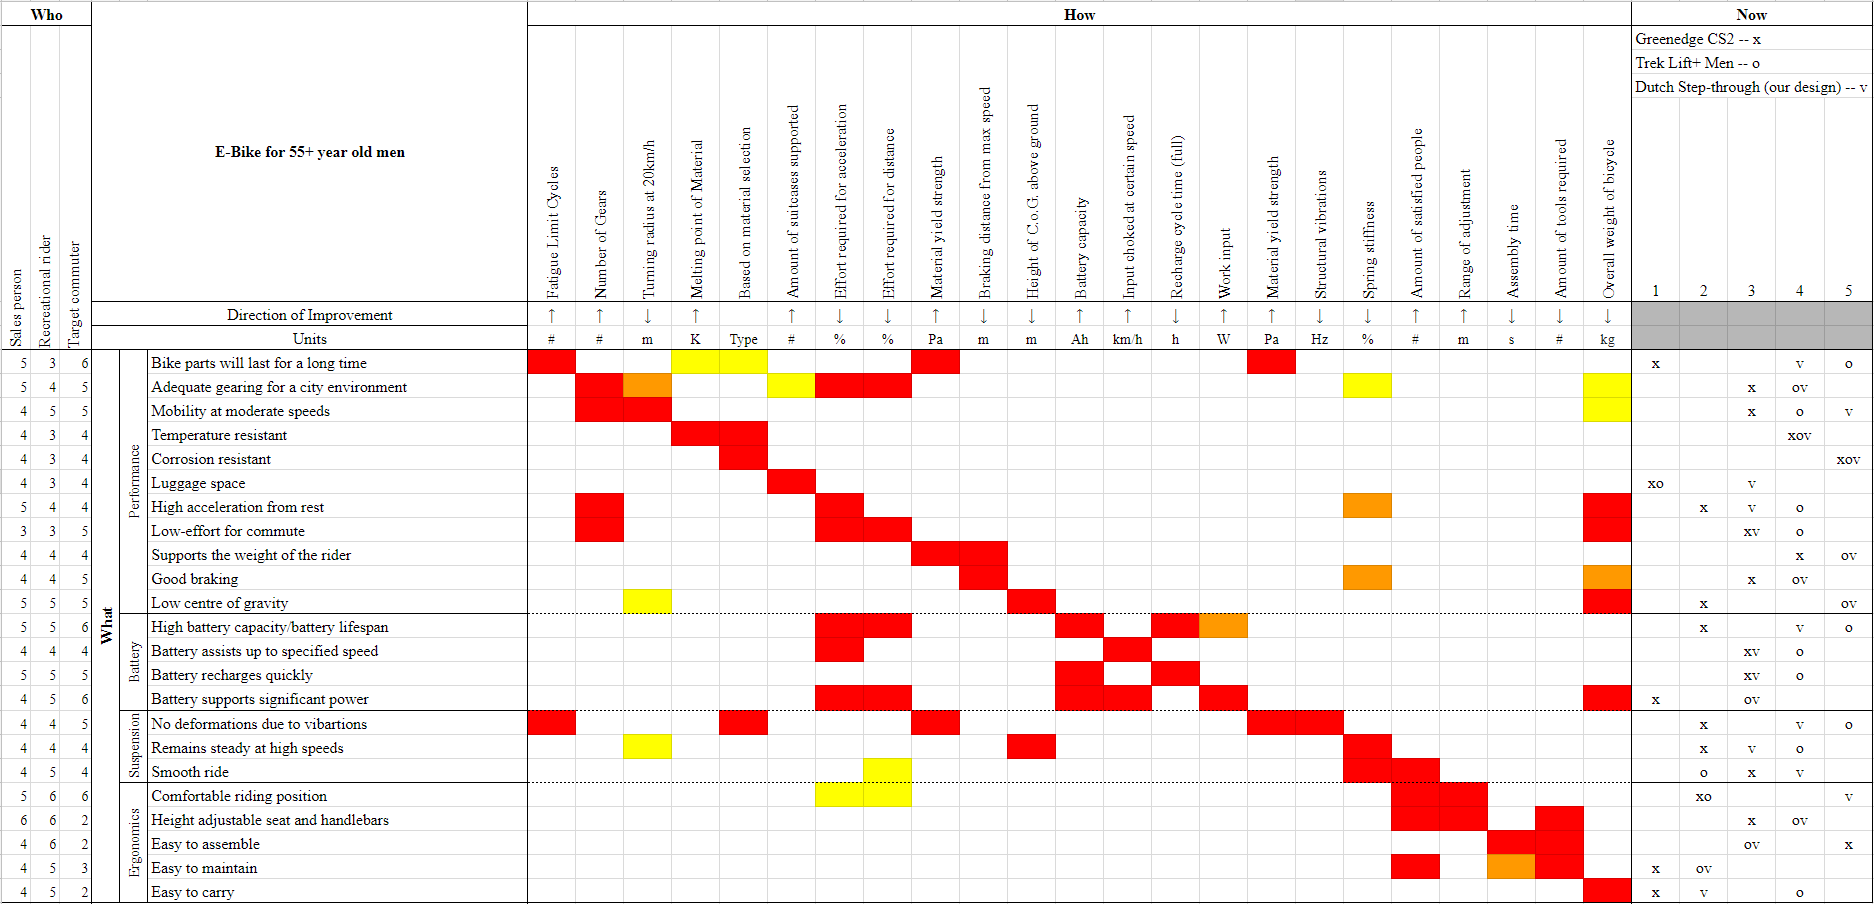
\includegraphics[width=1.45\textwidth]{Hoq}
\end{table}

\end{landscape}
\restoregeometry

\section{Detailed Design}

\subsection{Components}

\subsection{Material Selection}

\subsection{Calculations}

\subsection{Standards Considered}

\section{Costing and Implementation}

The intended product price from the Product Design Specification is between \textsterling1,700 and \textsterling2,200. This price range was selected to be competitive in the e-bike market, by being placed slightly over the average price. Additionally, it is expected that the designed e-bike would not have much competition due to this being an undeveloped market; classic e-bikes as opposed to sport e-bikes. 

The calculations are based on an assumption, where a new product is being developed for a large company. Therefore, the overheads will not be considered as the bike will be one of their many products. Furthermore, all the hardware and software have already been purchased. 

\[
	\text{Selling Price} = \text{Profit} + \left(\text{Works Cost Price} + \left(\frac{\text{Cost of Design}}{\text{Quantity}}\right)\right)
\]

\subsection{Cost of Design}

The cost of design describes the price which is invested into each bicycle. This includes the design labour (i.e. the hours spent by engineers directly working on the product), and the cost of the design material. Values for these are provided in the tables below.

\begin{table}[!ht]
	\centering
	\caption{Specific and total design labour cost}
	\begin{tabular}{l r r r}
		\hline
		\multicolumn{1}{l}{Tasks}&\multicolumn{1}{l}{Hours (h)}&\multicolumn{1}{l}{Cost per Hour (\textsterling/h)}&\multicolumn{1}{l}{Total Cost (\textsterling)}\\\hline
		Developing PDS	&3&20.00&60.00\\
		Initial Research&20&20.00&400.00\\
		Market Analysis&6&20.00&120.00\\
		Component Selection&8&20.00&160.00\\
		Material Selection&6&20.00&120.00\\
		Morphological Analysis&3&20.00&60.00\\
		Biomechanical Analysis&5&20.00&100.00\\
		CAD&20&20.00&400.00\\
		Further Development&100&20.00&2000.00\\
		FEA Simulation&20&20.00&400.00\\
		Component Testing&200&20.00&4000.00\\
		Drive Testing&20&10.00&200.00\\\hline
		Total&411&&8020.00\\\hline
	\end{tabular}
\end{table}

\begin{table}[!ht]
	\centering
	\caption{Specific and total design material costs}
	\begin{tabular}{l l r r}
		\hline
		\multicolumn{1}{l}{Component}&\multicolumn{1}{l}{Specification}&\multicolumn{1}{l}{Quantity}&\multicolumn{1}{l}{Total Cost (\textsterling)}\\\hline
		Motor&Bosch ActiveLine 250W BLDC&1&250.00\\
		Battery&Bosch Powerpack 300Wh (40 km range)&1&400.94\\
		Charger&Bosch Charger 4A&1&100.00\\
		Front Suspension&SR Suntour XCR-RL Fork Suspension&1&114.95\\
		Back Suspension&M2R Rear Schock Absorber 270mm&1&40.00\\
		Frame&7005-T6 Aluminium (Age Hardening) - 1500g&1&2.93\\
		Wheel&Cast Aluminium - 800g&2&3.12\\
		Tyre&Schwalbe Marathon GreenGuard City (26 in)&2&17.99\\
		Wheel Hub&Cast Aluminium - 300g&2&1.17\\
		Seat&Bioflex Websprung Gents Comfort&1&19.96\\
		Handlebar&Aluminium and Leather Coated&1&25.00\\
		Chain&Shimano HG93 (9 speed) Roller Chain&1&10.99\\
		Headlight&Bobbin Retro Front Light&1&19.99\\
		Brakes&Clarks CMD-11 Mechanical Brake Disc + Rotor&2&11.99\\
		Brake Handles&Shimano BL M425 Acera Brake Lever&2&14.44\\
		Cables&Shimano PTFE Coated Stainless Steel Wire&1&6.99\\
		Pannier Rack&Tortec Velocity Rear Pannier Rack - Silver&1&21.59\\
		Mudguard&SKS Bluemels Mudguard Set&1&25.38\\\hline
		Total&&&1087.43\\\hline
	\end{tabular}
\end{table}

Here, retail prices have been taken for components. Therefore, the worst-case scenario is being portrayed. In the case where wholesale prices were to be obtained from the providers, the total cost is expected to drop anywhere from 10\% to 20\%. 

\newpage

\subsection{Works Cost Price}

The Works Cost Price includes the price for the salaries of workers which are involved in building the bicycle. Hence, it must include welding costs, casting costs, assembly costs, and testing costs per bike. 

\begin{table}[!ht]
	\centering
	\caption{Specific and total works cost price per bike}
	\begin{tabular}{l r r r}
		\hline
		\multicolumn{1}{l}{Process}&\multicolumn{1}{l}{Hours (h)}&\multicolumn{1}{l}{Cost per hour (\textsterling/h)}&\multicolumn{1}{l}{Total Cost (\textsterling)}\\\hline
		Mechanical Assembly&2&15.00&30.00\\
		Electrical Wiring&1&15.00&15.00\\
		Gas Metal Arc (MIG) Welding&1&30.00&30.00\\
		Low Pressure Die Casting&1&5.00&5.00\\
		Testing&2&20.00&40.00\\\hline
		Total&7&&120.00\\\hline
	\end{tabular}
\end{table}

\subsection{Final Cost}

Assuming a worst-case scenario where only 100 e-bikes are sold in the first year, the retail price is calculated below assuming a healthy 50\% profit margin. 

\[
	\text{Selling Price} = 1.5 \times \left(1087.43+120.00+\frac{8020.00}{100}\right) =\text{\textsterling}1,931.45
\]

This leads to a net profit of \textsterling 643.82 per bike.

Although this is an elevated price, the following conclusions can be drawn. The cost of producing each bike is \textsterling 1287.63. This figure has been obtained without considering wholesale prices or economies of scale. Therefore, the total production cost could be expected to decrease by up to 30\%. Nonetheless, with the current information, the design fits within the price range specified in the PDS, whilst maintaining a profit margin of 50\%. With a maximum profit margin of 80\%. 

The final selling price can be determined once further market analysis and focus groups are conducted, to understand the current tendencies in the market. 

\subsection{Break Even Analysis}

The following is the break-even analysis conducted for the costs and prices which have been laid out in the above sections. It was also assumed that for the given production capacity, there would be three employees working full time at a standard wage of \textsterling 23,333 per annum.

\begin{figure}[ht]
	\caption{Graph displaying the break-even analysis. Break even achieved after 108 units sold.}
\end{figure}

\subsection{Profit and Loss Accounts}

The profit and loss accounts have been created for the first three years of the forecasted sales. The expected sales considered as a possibility throughout the first year are 100, 1,000 and 10,000; and a profit and loss account has been calculated for each individually. It was assumed that the number of full time employees required to manufacture 100 bicycles per year were 3, each having a salary of \textsterling 23,333 per annum (total of \textsterling 70,000). 30 were required for 1,000 bicycles (total of \textsterling 700,000), and 300 for 10,000 bicycles (total of \textsterling 7,000,000). Furthermore, the first year presented two extra costs. This included: design labour costs of \textsterling 8,200 and tooling costs of \textsterling 100,000. They are paid off in the first year and from then on, are not considered again. 

Taking a conservative approach, a contingency of \textsterling 10,000 was included for every 100 bicycles produced. Finally, a 20\% discount for raw materials was assumed for the 1,000-purchase situation, whilst a 30\% discount was assumed for the 10,000 units calculation. 

The profit and loss accounts are shown in Table~\ref{tab:PLA} below. Due to the healthy, and comfortable, 50\% profit margin imposed on the selling price, only three of the nine considered years would result in a negative profit, with two of them being a minimum loss of \textsterling 7,743. Therefore, it can be concluded that the product has enough of a profit margin while maintaining a competitive selling price. Additionally, the initial cost projection stated in the PDS has been met in the final design.  

\begin{table}[!ht]
	\centering
	\caption{Expected Profit and Loss accounts for units sold over the first three years}
	\begin{tabular}{l r r r r r r}	
		\hline
		Profit \& Loss Account Y1&\multicolumn{1}{l}{No.}&\multicolumn{1}{l}{\textsterling}&\multicolumn{1}{l}{No.}&\multicolumn{1}{l}{\textsterling}&\multicolumn{1}{l}{No.}&\multicolumn{1}{l}{\textsterling}\\ \hline
		Units Sold at \textsterling 1,930.00&100&193,000.00&1,000&1,930,000.00&10,000&19,300,000.00\\
		Costs of Sales at \textsterling 1,207.43&&120,743&&965,944&&8,452,010\\
		Total Direct Costs&&78,020.00&&708,020.00&&7,008,020.00\\
		Gross Margin&&-5,763.00&&256,036.00&&3,839,970.00\\
		Contingency (with tools)&&110,000.00&&200,000.00&&1,100,000.00\\
		Net Profit/Loss before Tax&&-115,763.00&&56,036.00&&2,739,970.00\\ \hline
		Profit \& Loss Account Y2&\multicolumn{1}{l}{No.}&\multicolumn{1}{l}{\textsterling}&\multicolumn{1}{l}{No.}&\multicolumn{1}{l}{\textsterling}&\multicolumn{1}{l}{No.}&\multicolumn{1}{l}{\textsterling}\\ \hline
		Units Sold at \textsterling 1,930.00&100&193,000.00&1,000&1,930,000.00&10,000&19,300,000.00\\
		Costs of Sales at \textsterling 1,207.43&&120,743&&965,944&&8,452,010\\
		Total Direct Costs&&70,000.00&&700,000.00&&7,000,000.00\\
		Gross Margin&&2,257.00&&264,056.00&&3,847,990.00\\
		Contingency&&10,000.00&&100,000.00&&1,000,000.00\\
		Net Profit/Loss before Tax&&-7,743.00&&164,056.00&&2,847,990.00\\ \hline
		Profit \& Loss Account Y3&\multicolumn{1}{l}{No.}&\multicolumn{1}{l}{\textsterling}&\multicolumn{1}{l}{No.}&\multicolumn{1}{l}{\textsterling}&\multicolumn{1}{l}{No.}&\multicolumn{1}{l}{\textsterling}\\ \hline
		Units Sold at \textsterling 1,930.00&100&193,000.00&1,000&1,930,000.00&10,000&19,300,000.00\\
		Costs of Sales at \textsterling 1,207.43&&120,743&&965,944&&8,452,010\\
		Total Direct Costs&&70,000.00&&700,000.00&&7,000,000.00\\
		Gross Margin&&2,257.00&&264,056.00&&3,847,990.00\\
		Contingency&&10,000.00&&100,000.00&&1,000,000.00\\
		Net Profit/Loss before Tax&&-7,743.00&&164,056.00&&2,847,990.00\\
	\end{tabular}
	\label{tab:PLA}
\end{table}

\subsection{Return on Investment}

The return on investment (ROI) has been calculated for each year of each of the three expected sales scenarios. The results are shown in Table~\ref{tab:ROI} below. 

The scenario where 100 bikes are sold never quite becomes profitable. The ROI does improve significantly over the first three years, however, from then on it will tend to a value slightly smaller than one over the years. Therefore, this would require for a slightly higher profit margin. However, the 1,000 bikes sold scenario has a steady increase in ROI, which although not big, still accounts for a 7.11\% improvement over the first three years. Therefore, the selling price is well selected for this situation. On the other hand, the 10,000 units sold scenario has a very big initial ROI with a very slight increase over the years. As a result, the profit margin should be decreased to attract more customers and establish the brand better within the market. 

\begin{table}[!ht]
	\centering
	\caption{Cumulative ROI over the first three years of Product launch}
	\begin{tabular}{r r r r}
		\hline
		\multicolumn{1}{l}{Year}&\multicolumn{1}{l}{100 Units Sold ROI}&\multicolumn{1}{l}{1,0000 Units sold ROI}&\multicolumn{1}{l}{10,000 Units sold ROI}\\ \hline
		1&0.6251&1.0299&1.1655\\
		2&0.7576&1.0605&1.1693\\
		3&0.8152&1.0711&1.1705\\
	\end{tabular}
	\label{tab:ROI}
\end{table}

\section{Project Evaluation}

\bibliographystyle{apacite}
\bibliography{References}

\end{document}
